\begin{frame}
    \frametitle{Explanation by Example}
    \begin{itemize}
        \gitem Nodes
    \end{itemize}
    \vspace{10.8pt}
    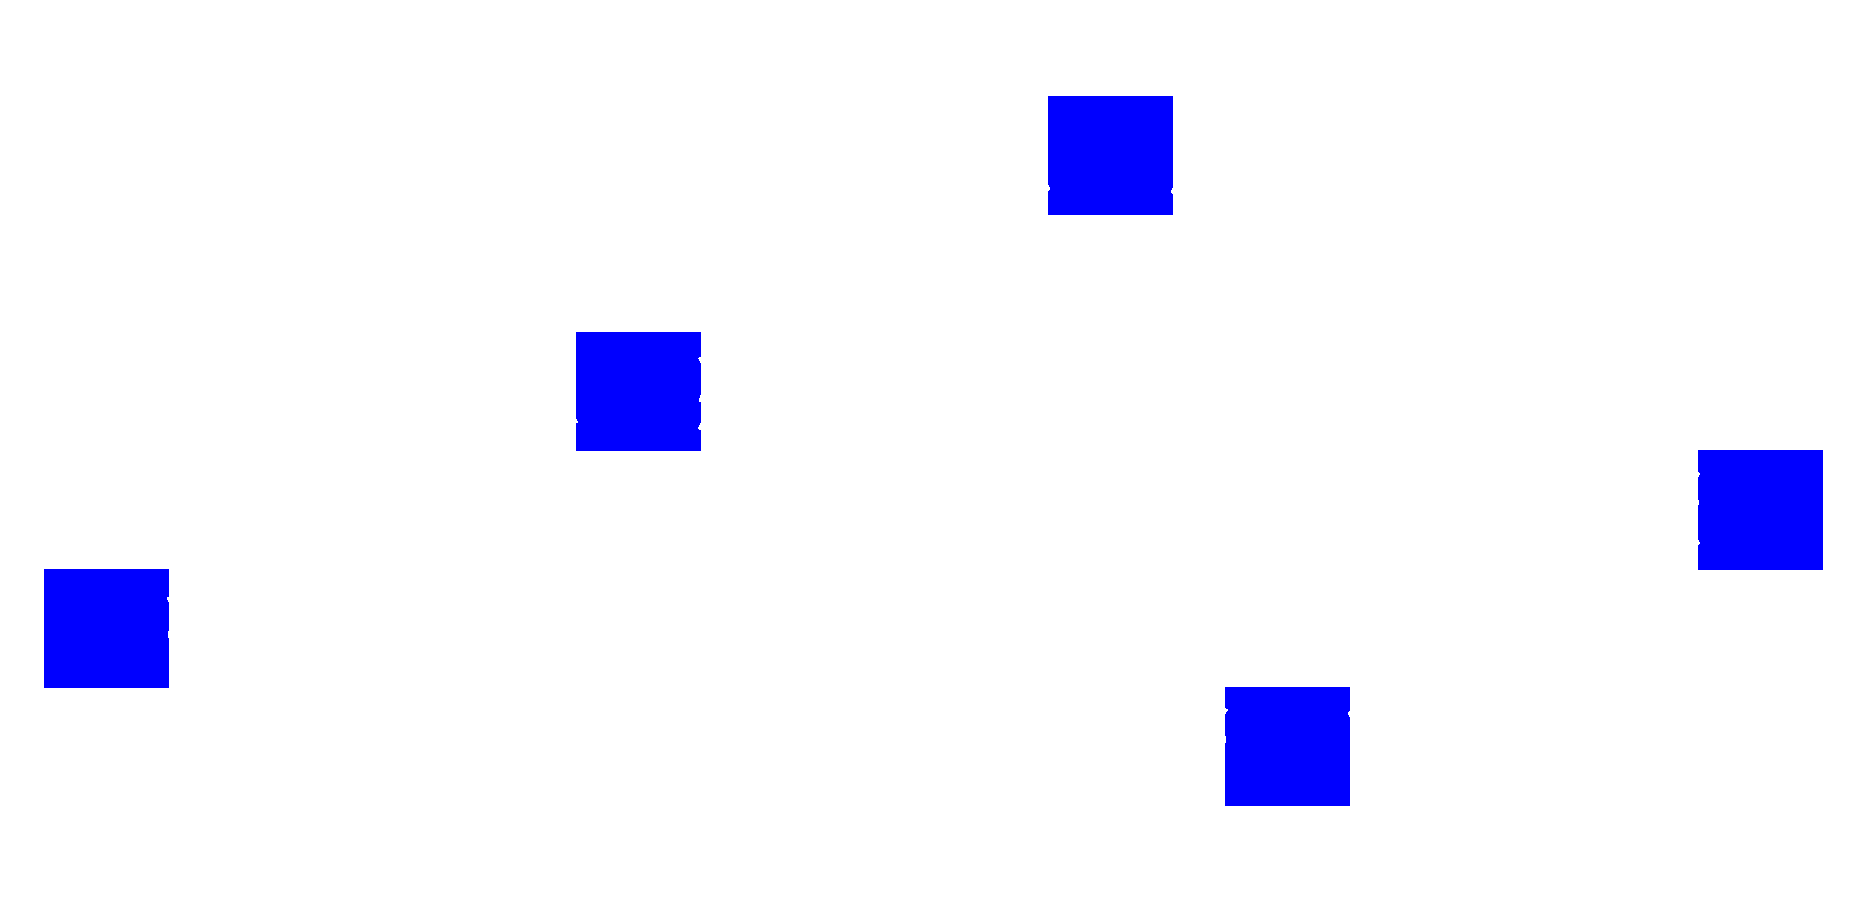
\includegraphics[width=\textwidth]{img/model1}
    \vfill
\end{frame}

\begin{frame}
    \frametitle{Explanation by Example}
    \begin{itemize}
        \gitem Observe $k$ Neighbors
    \end{itemize}
    \vspace{8.6pt}
    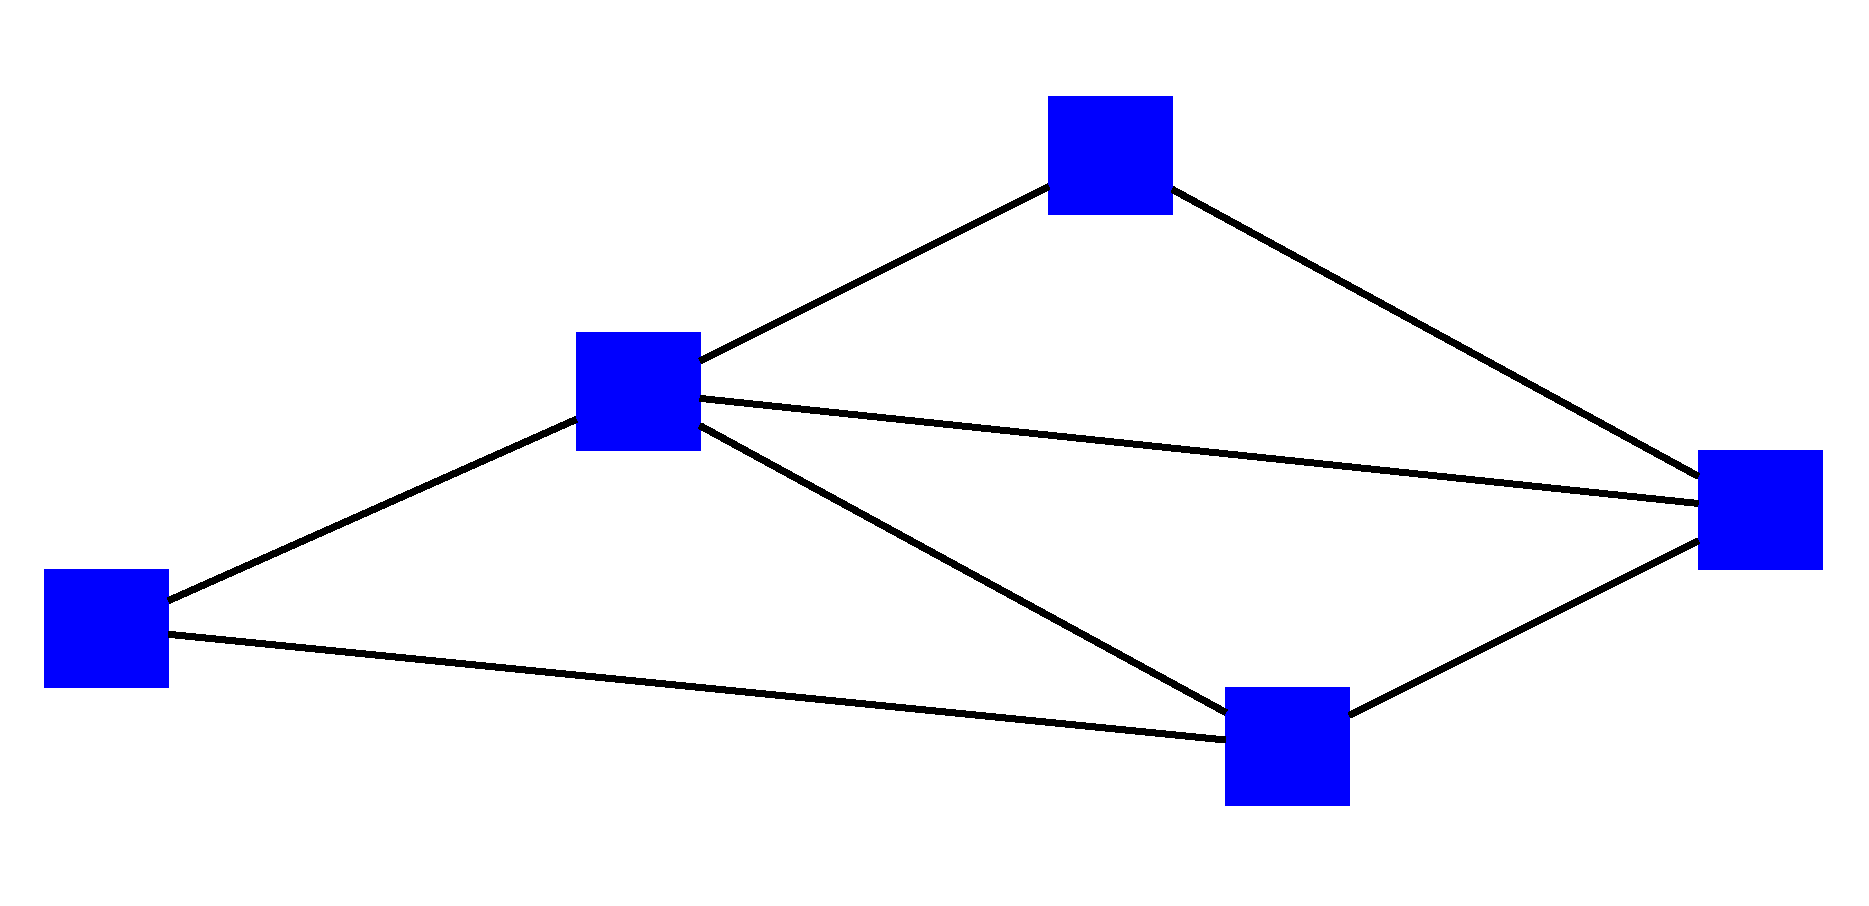
\includegraphics[width=\textwidth]{img/model2}
    \vfill
\end{frame}

\begin{frame}
    \frametitle{Explanation by Example}
    \begin{itemize}
        \gitem State $\in \lbrace 0, 1 \rbrace$
    \end{itemize}
    \vspace{8pt}
    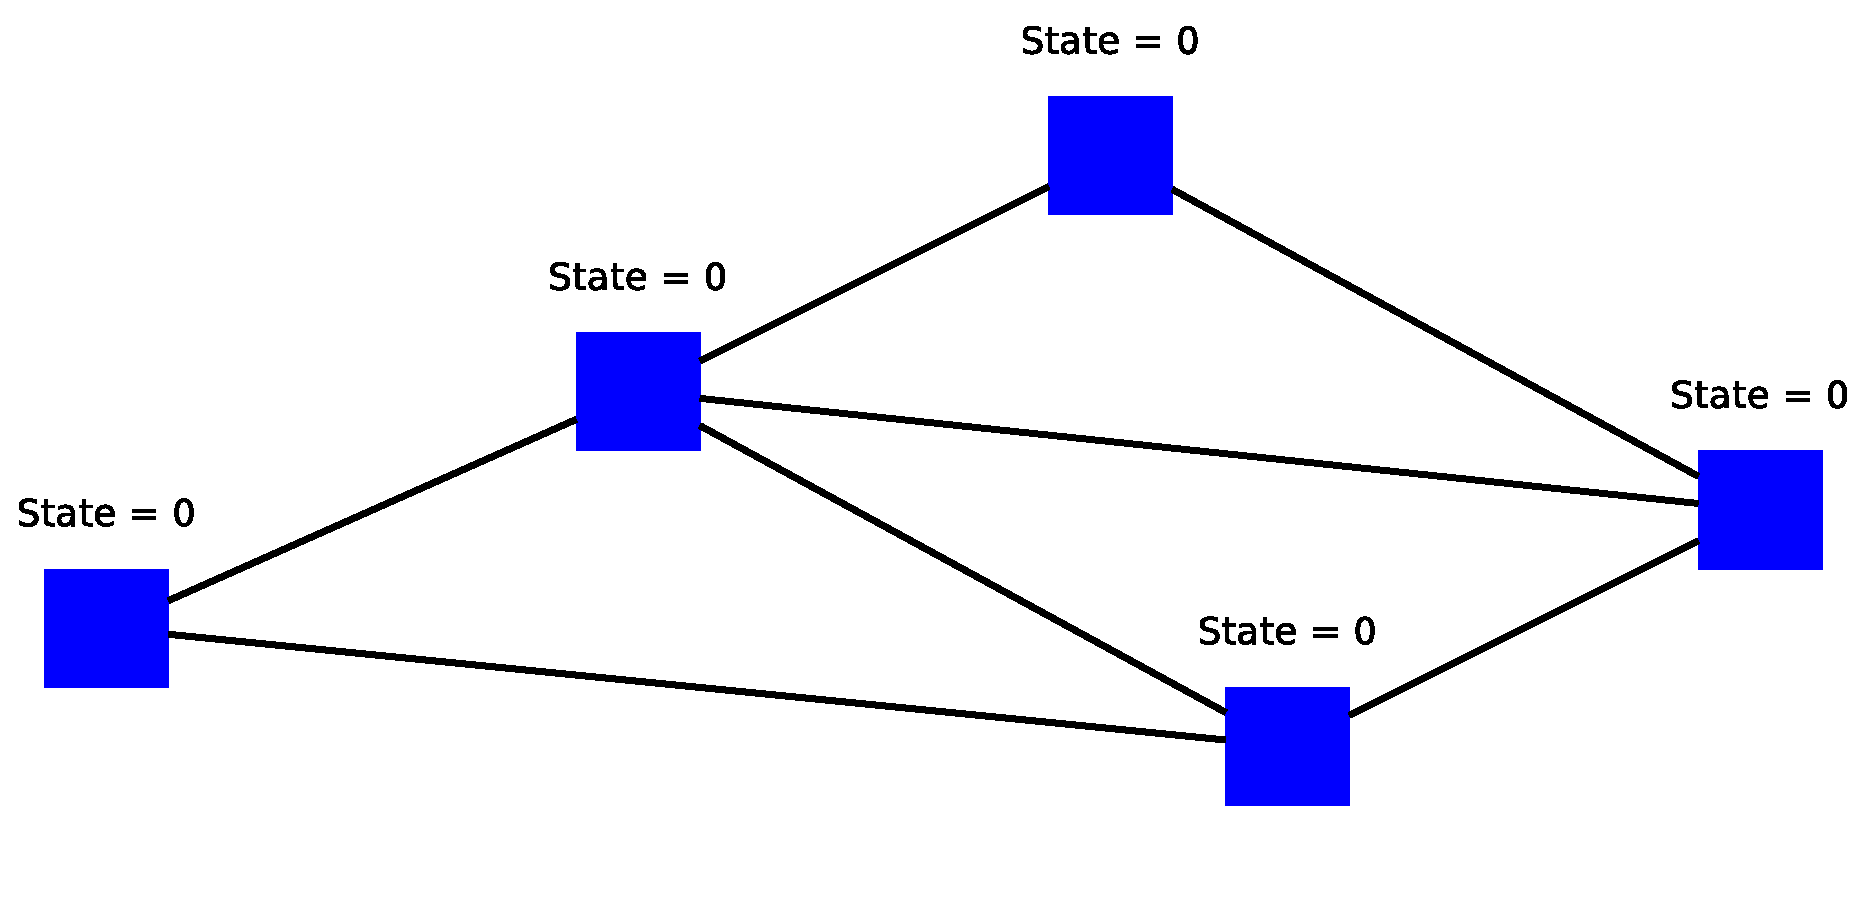
\includegraphics[width=\textwidth]{img/model3}
    \vfill
\end{frame}

\begin{frame}
    \frametitle{Explanation by Example}
    \begin{itemize}
        \gitem Threshold $\Phi \in [0, 1]$
    \end{itemize}
    \vspace{8pt}
    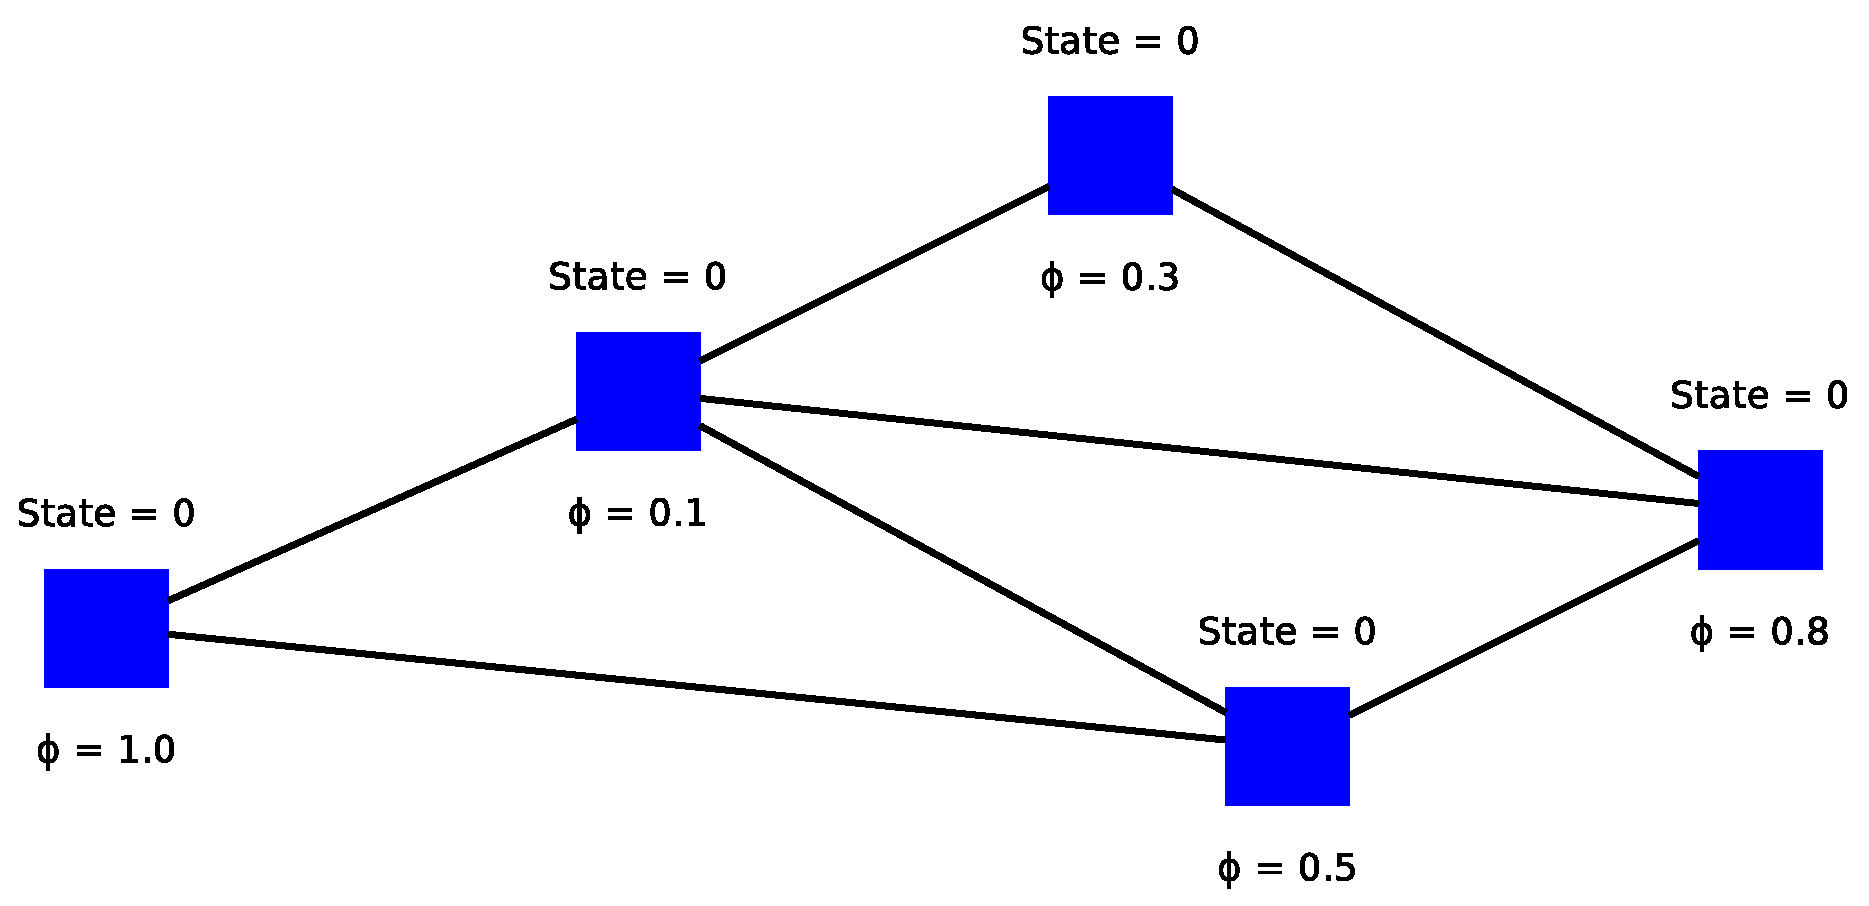
\includegraphics[width=\textwidth]{img/model4}
    \vfill
\end{frame}

\begin{frame}
    \frametitle{Explanation by Example}
    \begin{itemize}
        \gitem Random Impulse Happens
    \end{itemize}
    \vspace{8.6pt}
    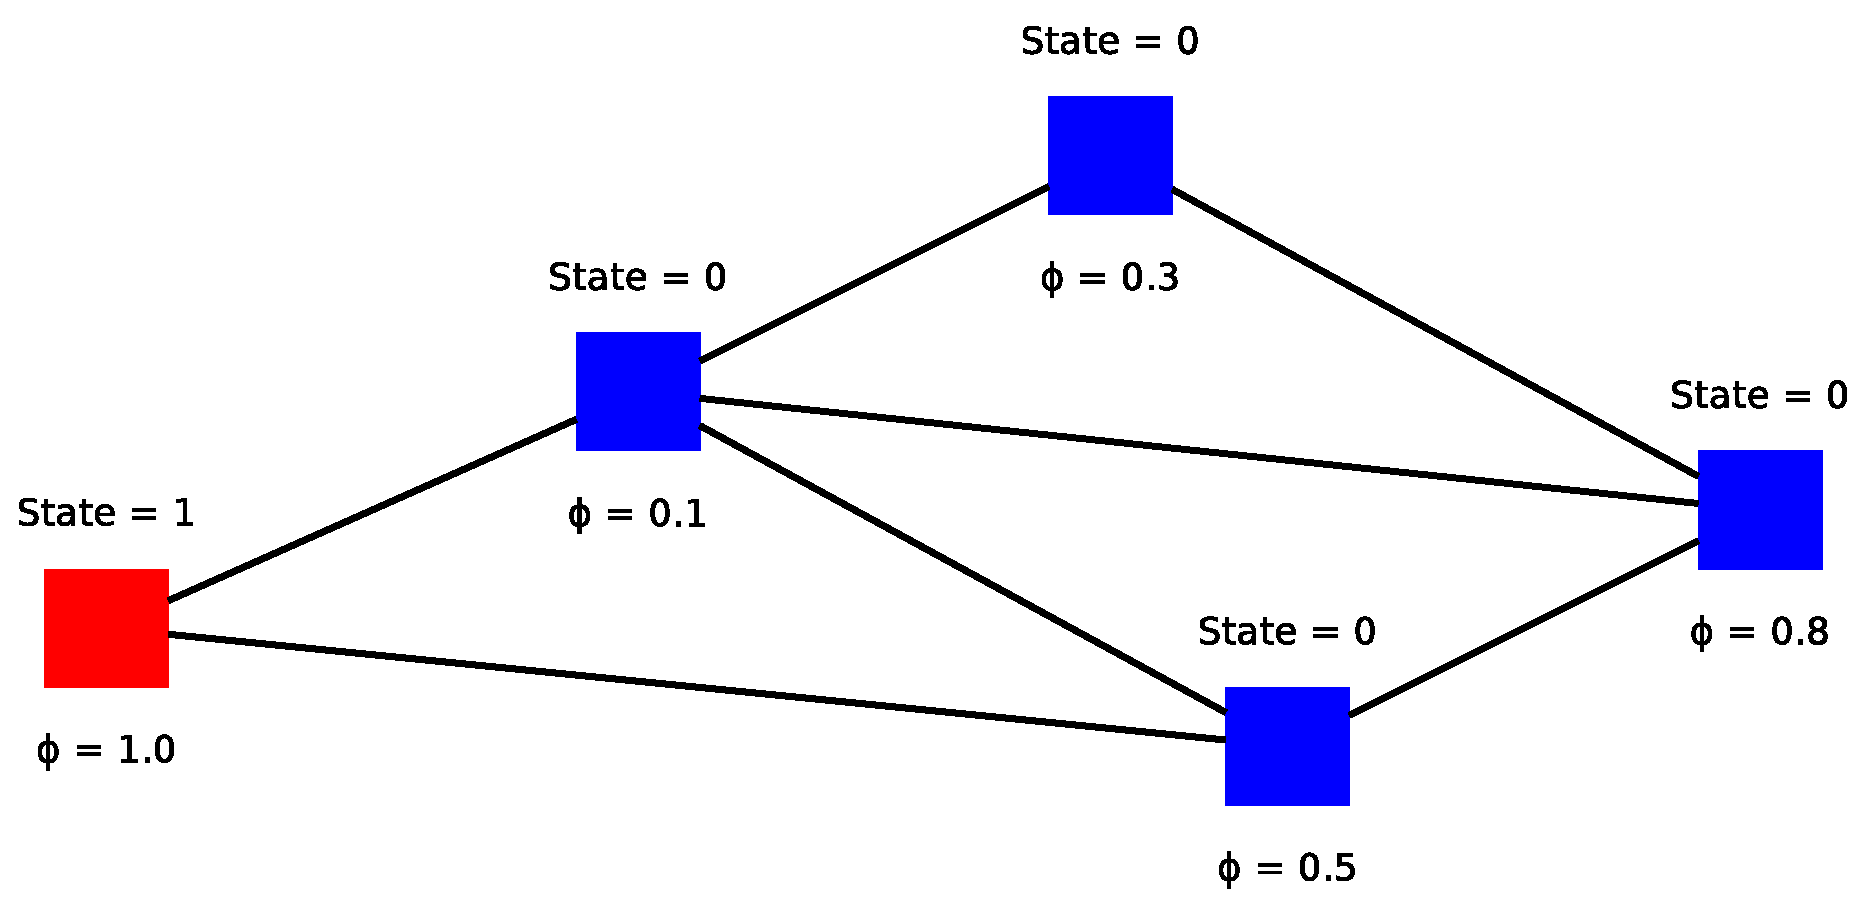
\includegraphics[width=\textwidth]{img/model5}
    \vfill
\end{frame}

\begin{frame}
    \frametitle{Explanation by Example}
    \begin{itemize}
        \gitem Nodes Check in Random Intervals
    \end{itemize}
    \vspace{10.8pt}
    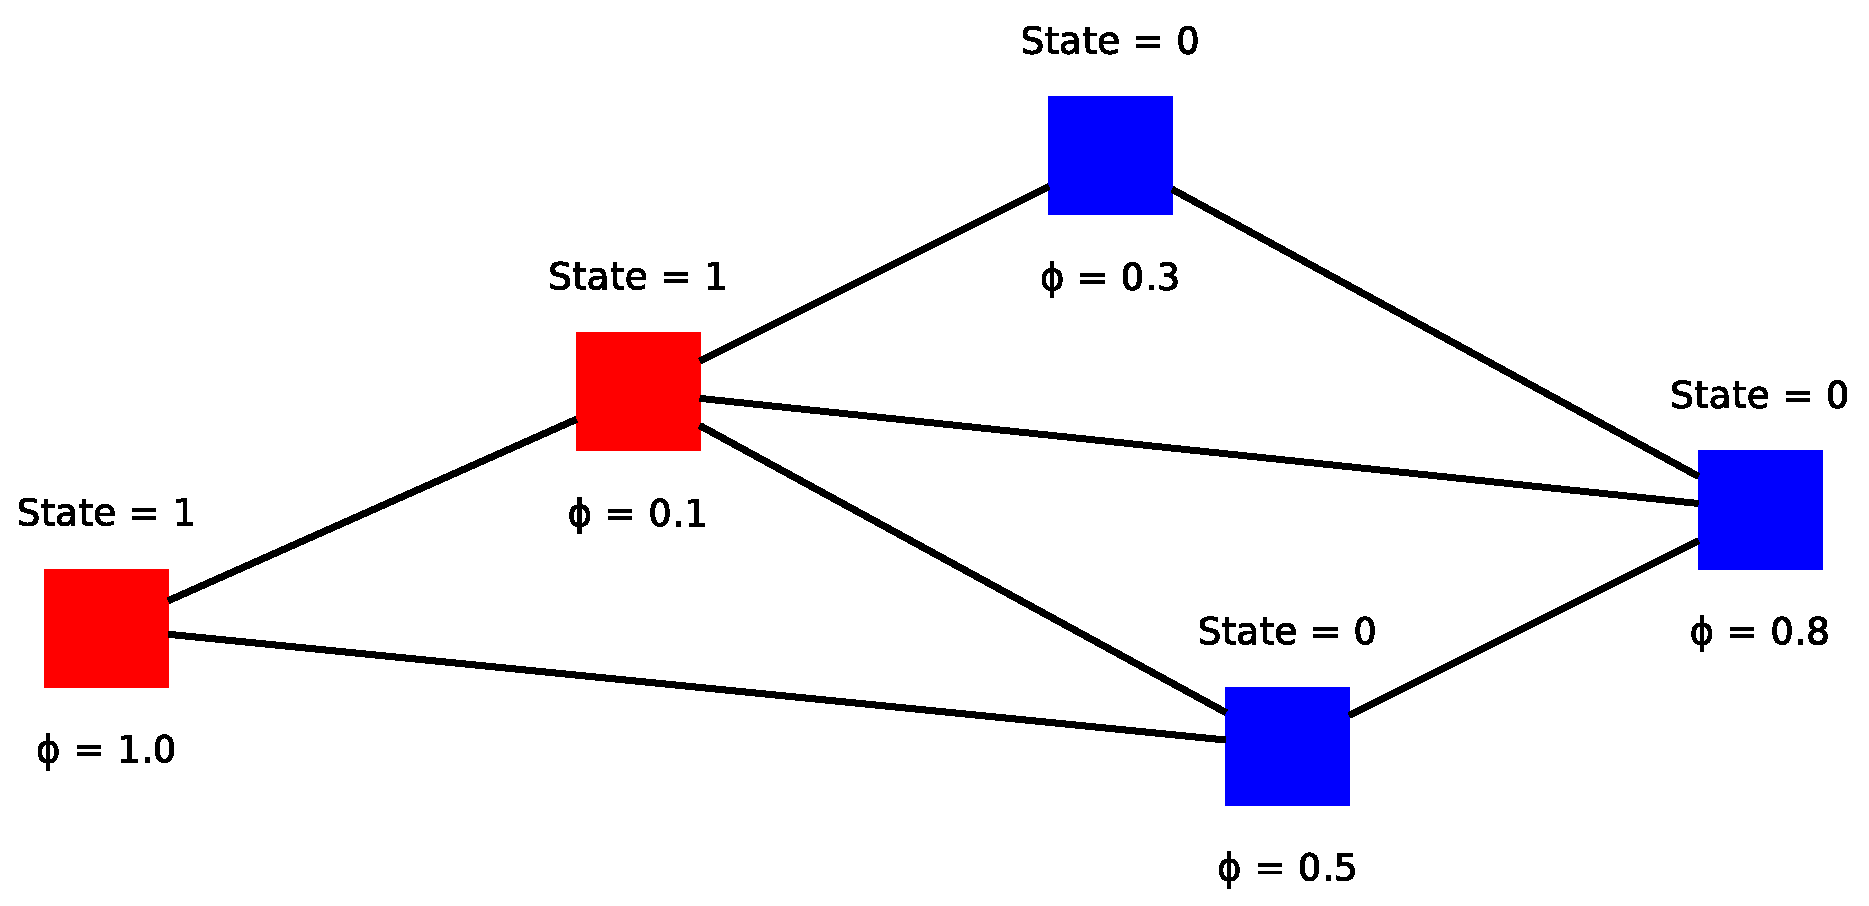
\includegraphics[width=\textwidth]{img/model6}
    \vfill
\end{frame}

\begin{frame}
    \frametitle{Explanation by Example}
    \begin{itemize}
        \gitem Stuff Happens
    \end{itemize}
    \vspace{8.8pt}
    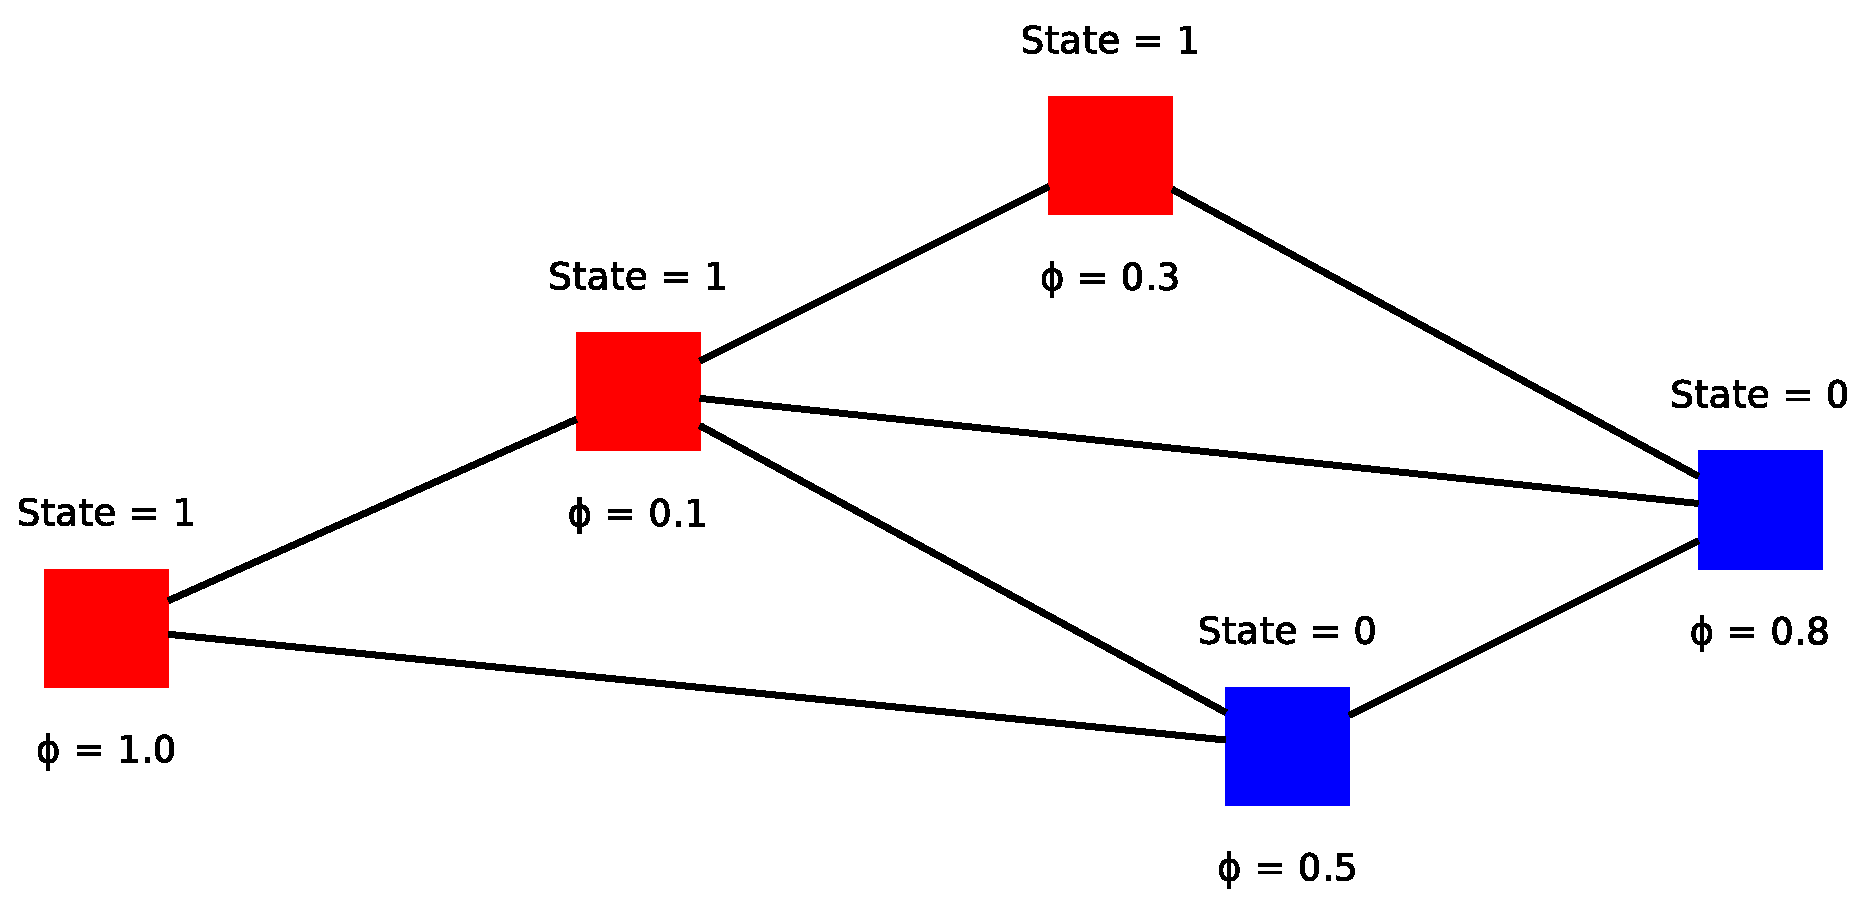
\includegraphics[width=\textwidth]{img/model7}
    \vfill
\end{frame}

\begin{frame}
    \frametitle{Explanation by Example}
    \begin{itemize}
        \gitem Things Occur
    \end{itemize}
    \vspace{8.8pt}
    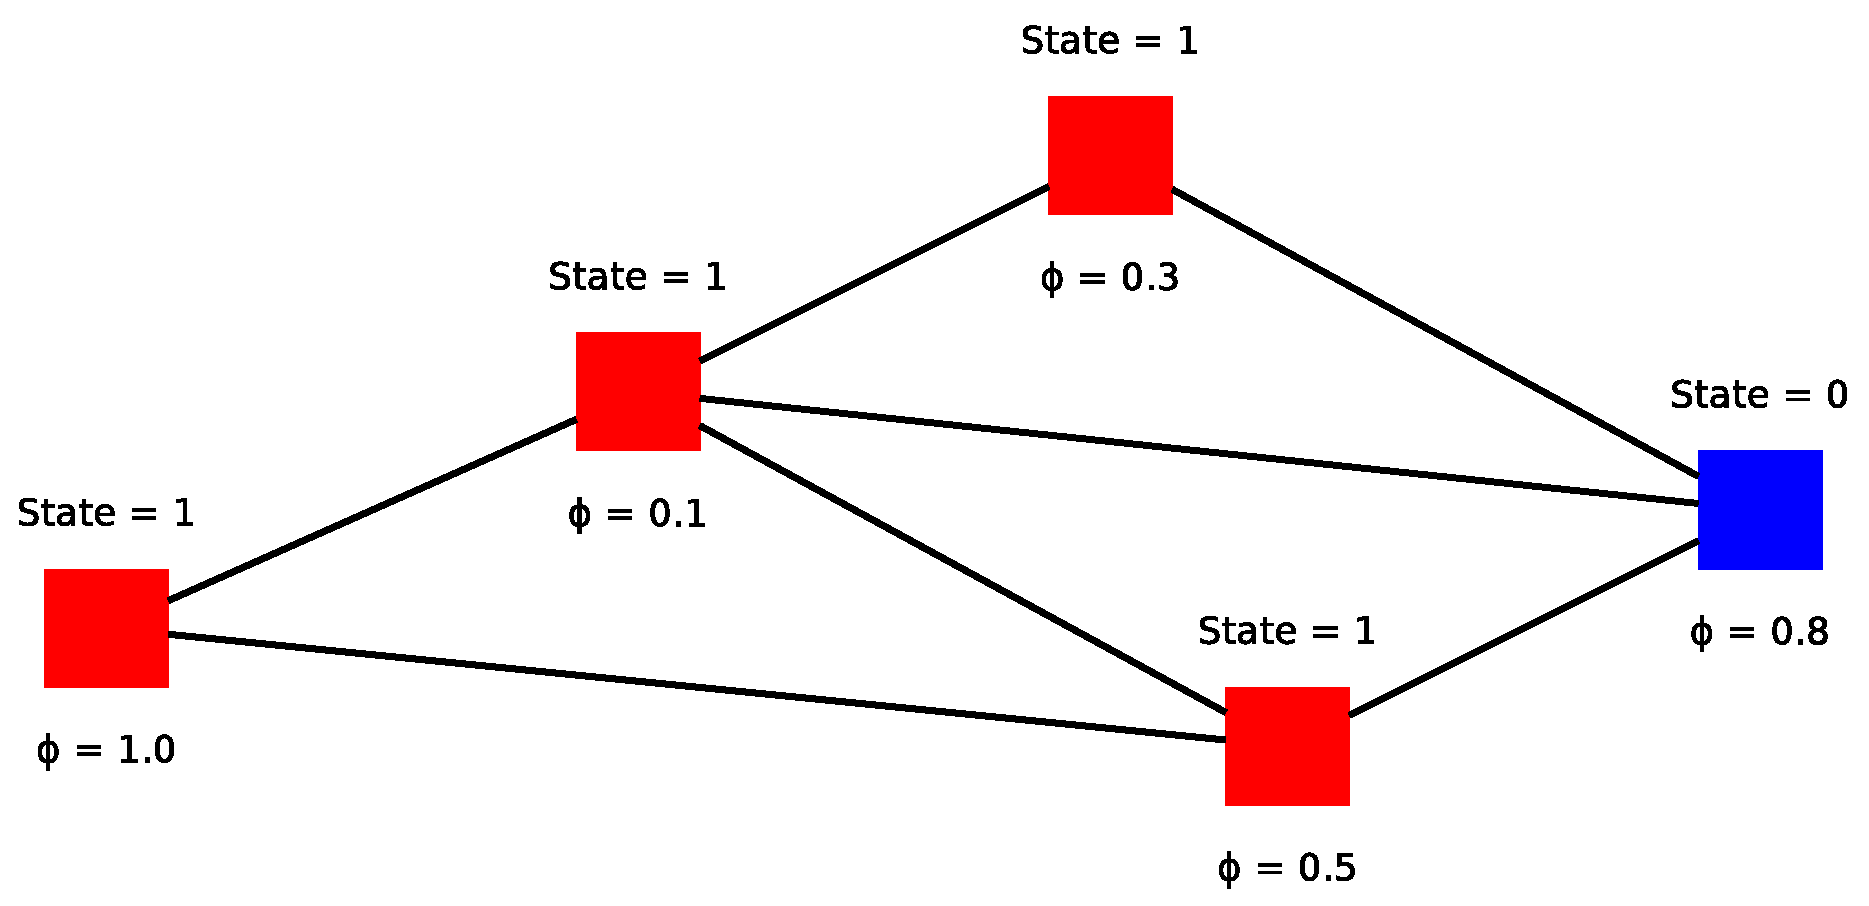
\includegraphics[width=\textwidth]{img/model8}
    \vfill
\end{frame}

\begin{frame}
    \frametitle{Explanation by Example}
    \begin{itemize}
        \gitem Coup Successful
    \end{itemize}
    \vspace{8.8pt}
    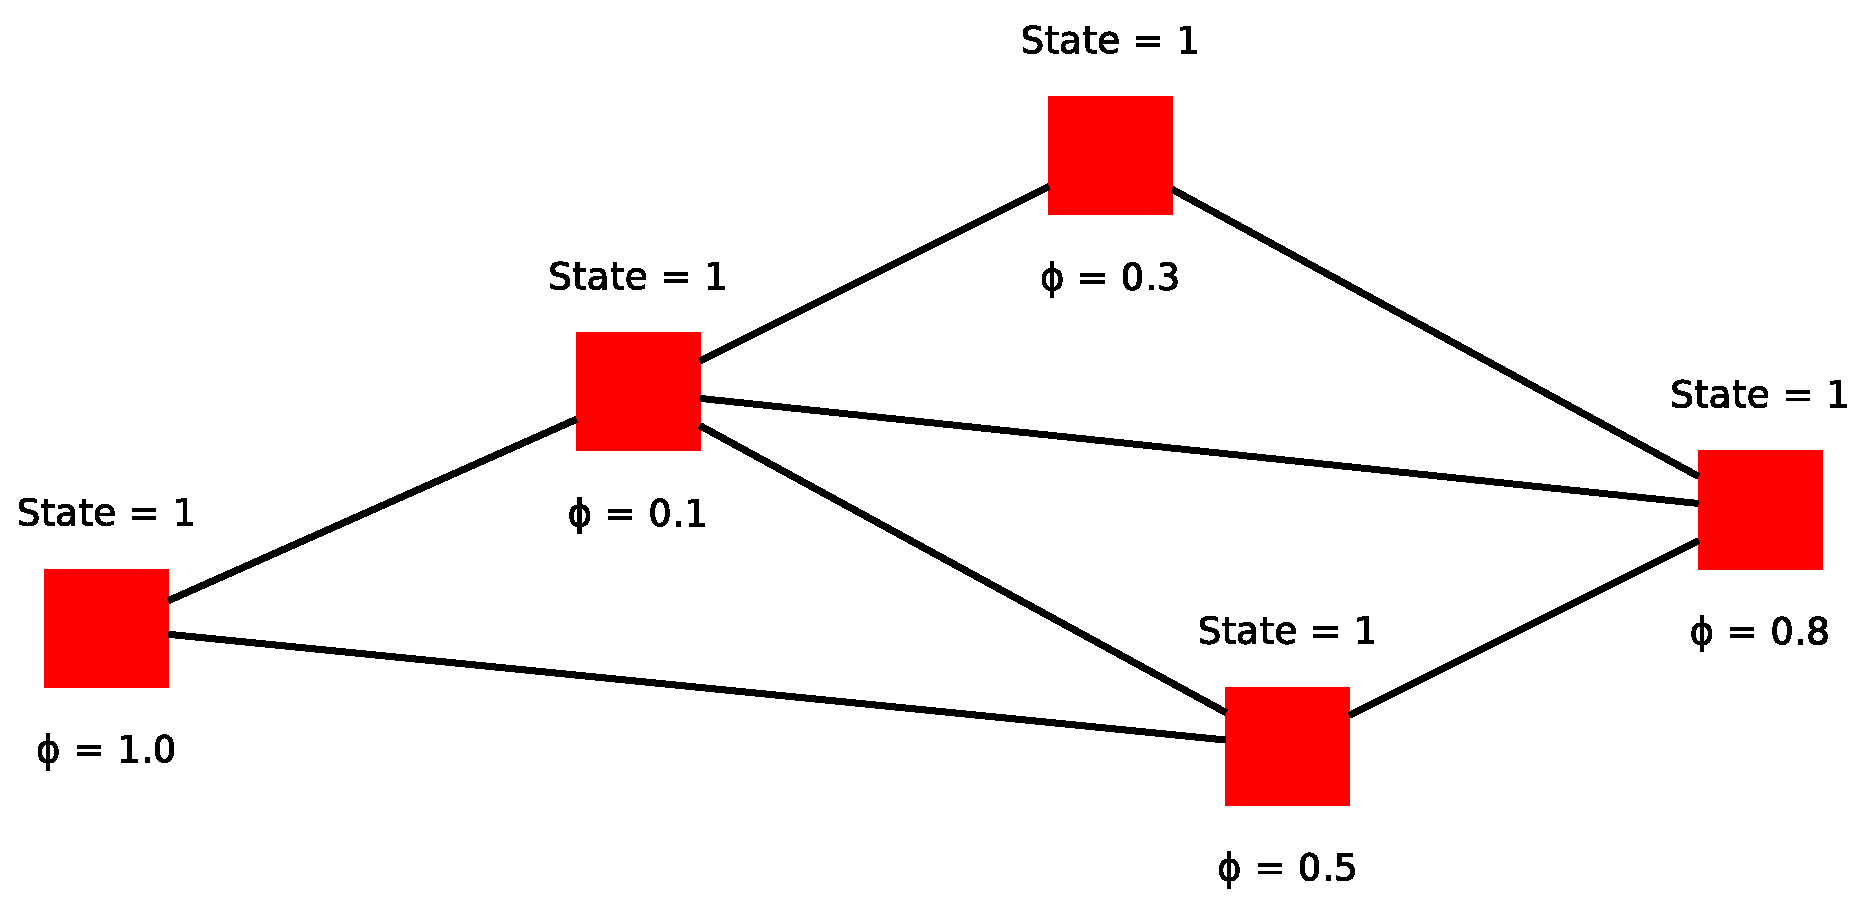
\includegraphics[width=\textwidth]{img/model9}
    \vfill
\end{frame}
